\documentclass[twocolumn,pra,aps,superscriptaddress,floatfix,10pt]{revtex4-2}

\usepackage{amsmath}
\usepackage{graphicx}
\usepackage{xcolor}
\usepackage{bm}
\usepackage[colorlinks=true,linkcolor=black,citecolor=black,urlcolor=blue]{hyperref}

\begin{document}

\title{Magnetic field inhomogeneity as a systematic bias in ground-state positronium hyperfine structure measurements}

\author{Ernest Darell Zermeno}
\email{0244552@up.edu.mx}
\affiliation{Universidad Panamericana, Guadalajara, M\'exico}

\date{\today}

\begin{abstract}
The ground-state hyperfine structure (HFS) interval of positronium has shown a persistent $3.9\sigma$ discrepancy between the weighted average of the 1983--1984 measurements ($203\,388.65 \pm 0.67$\,MHz) and the QED prediction ($203\,391.69 \pm 0.41$\,MHz). We quantify for the first time the systematic bias introduced by magnetic field inhomogeneity in these measurements. Using the field gradients measured and published by Mills \& Bearman ($\partial^2 B/\partial z^2 = +44$\,ppm/cm$^2$, $\partial^2 B/\partial r^2 = -21$\,ppm/cm$^2$) and the actual cavity dimensions and positronium spatial distributions from the original publications, we numerically reproduce the complete experimental procedure and find a bias of $\delta\Delta_\mathrm{HFS} = -0.22$\,MHz for the Mills measurement. For the Ritter measurement, using the reported post-shimming field uniformity, the bias is $-0.18$ to $-0.30$\,MHz. Combined with the $\sim 2$\,MHz non-thermalization correction identified by Ishida \textit{et~al.}, these previously unquantified systematics reduce the discrepancy from $3.9\sigma$ to approximately $1.5\sigma$. The superconducting magnet of Ishida \textit{et~al.} (0.9\,ppm uniformity) gives $|\delta\Delta_\mathrm{HFS}| < 0.2$\,MHz, consistent with their agreement with QED. A self-consistent treatment combining field inhomogeneity and thermalization dynamics, which we identify as necessary future work, could further reduce or eliminate the residual tension.
\end{abstract}

\maketitle

%% ====================================================================
\section{Introduction}
\label{sec:intro}
%% ====================================================================

Positronium (Ps), the bound state of an electron and a positron, is the lightest purely leptonic atom and provides a uniquely clean system for testing bound-state quantum electrodynamics (QED)~\cite{Adkins2022,Karshenboim2005}. Its ground-state hyperfine structure (HFS) interval---the splitting between the $1\,^3S_1$ (ortho-Ps) and $1\,^1S_0$ (para-Ps) levels---has been calculated to high precision within QED. The current theoretical prediction, including corrections through $O(m\alpha^6)$ and partial $O(m\alpha^7)$ contributions, is~\cite{Kniehl2000,Melnikov2001,Baker2014}
\begin{equation}
  \Delta_\mathrm{HFS}^\mathrm{QED} = 203\,391.69 \pm 0.41~\mathrm{MHz},
  \label{eq:qed}
\end{equation}
with the uncertainty dominated by uncalculated non-logarithmic $O(m\alpha^7)$ terms.

The two most precise experimental determinations of $\Delta_\mathrm{HFS}$ both employed the indirect Zeeman method in gas-filled microwave cavities within conventional electromagnets:
\begin{align}
  \Delta_\mathrm{HFS}^\mathrm{Mills} &= 203\,387.5 \pm 1.6~\mathrm{MHz}~\cite{Mills1975,Mills1983}, \\
  \Delta_\mathrm{HFS}^\mathrm{Ritter} &= 203\,389.10 \pm 0.74~\mathrm{MHz}~\cite{Ritter1984}.
\end{align}
The weighted average is $203\,388.65 \pm 0.67$\,MHz, yielding a discrepancy with theory of
\begin{equation}
  \delta\Delta_\mathrm{HFS} = -3.04 \pm 0.79~\mathrm{MHz}~(3.9\sigma).
  \label{eq:discrepancy}
\end{equation}

A more recent measurement by Ishida \textit{et~al.}~\cite{Ishida2014}, using a superconducting solenoid with 0.9\,ppm field uniformity, obtained $203\,394.2 \pm 2.1$\,MHz---consistent with QED at $1.2\sigma$ but with insufficient precision to definitively resolve the discrepancy. Ishida \textit{et~al.} identified incomplete thermalization of positronium as a systematic bias of approximately 10\,ppm ($\sim 2$\,MHz), which was not corrected in the earlier measurements.

The importance of cavity-related systematics has been underscored by recent work at UCL on positronium fine-structure measurements. Akopyan \textit{et~al.}~\cite{Akopyan2021} showed through numerical simulations that microwave reflections within the vacuum chamber produce frequency-dependent power distributions that distort spectral line shapes and shift extracted frequencies by several MHz. Sheldon \textit{et~al.}~\cite{Sheldon2023} confirmed this by redesigning the microwave environment, reducing a $4.5\sigma$ fine-structure discrepancy~\cite{Gurung2020} to $1.3\sigma$. These results demonstrate that electromagnetic environment effects within experimental cavities can produce MHz-level systematic shifts. The historical orthopositronium lifetime puzzle (1987--2003), eventually traced to incomplete thermalization and cavity wall effects~\cite{Vallery2003}, provides a cautionary precedent for the role of uncontrolled systematics in precision positronium measurements.

The possibility that magnetic field inhomogeneity constitutes a systematic error in the Zeeman-method HFS measurements has been recognized qualitatively for over a decade. Miyazaki~\cite{Miyazaki2010} identified field non-uniformity and non-thermalization as ``probable common systematic errors'' in all previous experiments. Asai \textit{et~al.}~\cite{Asai2012} noted the same concern in the context of developing a direct 203\,GHz measurement that avoids the static magnetic field entirely. The ETH Zurich group~\cite{Heiss2018} explicitly designed their experiment to be ``free of systematic effects found in earlier experiments, namely the inhomogeneity in static magnetic fields.'' However, no prior work has \emph{quantified} the magnitude of this bias using the actual experimental parameters. The present work provides this quantitative assessment.

In this work, we use the field gradients published by Mills \& Bearman~\cite{Mills1975}, together with the actual cavity dimensions and positronium distributions from the original experiments, to compute the systematic bias. The physical mechanism is straightforward: if the magnetic field varies across the cavity, different positronium atoms experience different local fields and thus different Zeeman splittings. The resulting resonance curve is a weighted average of individual Lorentzian responses. When the field distribution has a nonzero mean offset from the nominal value, the peak of the averaged resonance shifts, and the Breit-Rabi inversion yields a biased value of $\Delta_\mathrm{HFS}$.

%% ====================================================================
\section{Method}
\label{sec:method}
%% ====================================================================

\subsection{The indirect Zeeman method}
\label{sec:zeeman}

All three precision measurements of the ground-state HFS~\cite{Mills1975,Ritter1984,Ishida2014} used the indirect Zeeman resonance technique. Positrons from a $^{22}$Na source thermalize in a gas-filled cylindrical microwave cavity placed in a static magnetic field. The field mixes the $|1\,^1S_0\rangle$ (singlet) and $|1\,^3S_1, m=0\rangle$ (triplet) states, giving the mixed state a nonzero 2$\gamma$ annihilation rate. Microwaves at a fixed frequency $\nu_\mathrm{MW}$ drive transitions between the mixed state $|+\rangle$ (predominantly triplet $m=0$) and the $|1\,^3S_1, m=+1\rangle$ state. The magnetic field is swept through resonance, and the transition is detected as an increase in the 2$\gamma$ annihilation rate. The resonance field $B_\mathrm{res}$ is extracted from a Lorentzian fit to the signal curve, and $\Delta_\mathrm{HFS}$ is obtained by inverting the Breit-Rabi formula. Table~\ref{tab:experiments} summarizes the experimental parameters.

\begin{table}[b]
\caption{Experimental parameters for the three HFS measurements.}
\label{tab:experiments}
\begin{ruledtabular}
\begin{tabular}{lccc}
 & Mills~\cite{Mills1975} & Ritter~\cite{Ritter1984} & Ishida~\cite{Ishida2014} \\
\hline
$B_0$ (T) & 0.925 & 0.79 & 0.866 \\
$\nu_\mathrm{MW}$ (MHz) & 3253 & 2384 & 2856.6 \\
Cavity $R$ (mm) & 56.25 & 76.8 & 64 \\
Cavity $L$ (mm) & 12.7 & 38.1 & 100 \\
Magnet type & Electro. & Electro. & SC solenoid \\
$B$ uniformity & meas. & $\sim 0.5$\,ppm$^\dagger$ & 0.9\,ppm \\
\end{tabular}
\end{ruledtabular}
\footnotetext[1]{Post-shimming weighted standard deviation~\cite{Ritter1984}.}
\end{table}

\subsection{Positronium in a magnetic field}
\label{sec:hamiltonian}

The ground-state Hamiltonian of positronium in a magnetic field $B$ along $\hat{z}$ is
\begin{equation}
  H = H_\mathrm{HFS} + H_\mathrm{Z},
  \label{eq:hamiltonian}
\end{equation}
where $H_\mathrm{HFS} = (\Delta/4)\,\bm{\sigma}_e \cdot \bm{\sigma}_p$ is the hyperfine interaction and $H_\mathrm{Z} = g_e \mu_B B \,(S_{ez} - S_{pz})/\hbar$ is the Zeeman interaction. Here $g_e = 2.002\,319\,304$ is the electron $g$-factor and $\mu_B/h = 13\,996.245$\,MHz/T is the Bohr magneton in frequency units.

In the product basis $\{|\!\uparrow\uparrow\rangle, |\!\uparrow\downarrow\rangle, |\!\downarrow\uparrow\rangle, |\!\downarrow\downarrow\rangle\}$ (electron spin first), the Zeeman operator is diagonal with eigenvalues $(0, +1, -1, 0)$ in units of $g_e\mu_B B$. This reflects the fundamental property of positronium: the $m = \pm 1$ triplet states have $(S_{ez} - S_{pz}) = 0$ and are \emph{exactly unaffected} by the magnetic field. Only the $m = 0$ subspace is mixed. The eigenvalues are
\begin{align}
  E_{m=\pm 1} &= \Delta/4, \label{eq:Em1} \\
  E_{\pm} &= -\Delta/4 \pm \tfrac{1}{2}\sqrt{\Delta^2 + 4V^2}, \label{eq:Epm}
\end{align}
where $V = g_e \mu_B B$. The measured transition frequency is
\begin{equation}
  \nu_\mathrm{trans}(B) = E_+ - E_{m=+1} = \tfrac{\Delta}{2}\bigl(\sqrt{1 + x^2} - 1\bigr),
  \label{eq:nutrans}
\end{equation}
where $x = 2g_e\mu_B B/\Delta$. Figure~\ref{fig:zeeman} shows the four eigenvalues as a function of $B$. In our numerical implementation, we diagonalize the full $4 \times 4$ Hamiltonian matrix rather than using Eq.~(\ref{eq:nutrans}), which provides cross-validation.

\begin{figure}[htbp]
  \centering
  
\includegraphics[width=\columnwidth]{fig1_zeeman_eigenvalues.png}
  \caption{Zeeman eigenvalues of the positronium ground state as a function of magnetic field $B$. The four states are: $E_-$ (predominantly singlet, blue), $E_{m=\pm 1} = \Delta/4$ (triplet $m = \pm 1$, green/orange, exactly degenerate), and $E_+$ (predominantly triplet $m=0$, red). The vertical dashed line marks the Mills resonance field ($B_0 = 0.925$\,T). The purple arrow indicates the measured transition $E_+ - E_{m=+1}$.}
  \label{fig:zeeman}
\end{figure}

\subsection{Magnetic field profiles}
\label{sec:field_models}

For the Mills experiment, we use the field gradients directly measured and reported in Ref.~\cite{Mills1975}. NMR probe measurements at the cavity center yielded $\partial^2 B/\partial x^2 = -14$\,ppm/cm$^2$, $\partial^2 B/\partial y^2 = -28$\,ppm/cm$^2$, and $\partial^2 B/\partial z^2 = +44$\,ppm/cm$^2$, where $z$ is the field direction. In cylindrical symmetry, we use the azimuthal average $\partial^2 B/\partial r^2 = -21$\,ppm/cm$^2$. The field profile is then
\begin{equation}
  B(r,z) = B_0\left[1 + \frac{1}{2}\alpha_r r^2 + \frac{1}{2}\alpha_z z^2\right],
  \label{eq:mills_field}
\end{equation}
where $\alpha_r = -0.21$\,m$^{-2}$ and $\alpha_z = +0.44$\,m$^{-2}$ are the measured second derivatives in fractional units ($\delta B / B_0$ per m$^2$). This model has \emph{no free parameters}---it is fully determined by the published experimental data. For cylindrical pole-piece electromagnets, the field is strongest on the symmetry axis and decreases radially, corresponding to $\alpha_r < 0$~\cite{Rich1981}.

For the Ritter experiment, which used a Varian V4012A electromagnet (pole diameter 304.8\,mm, gap 66.7\,mm)~\cite{Theriot1970,Ritter1984} with careful shimming, we use a quadrupolar parameterization
\begin{equation}
  B(r,z) = B_0\left[1 + c_2\,\frac{2z^2 - r^2}{R_\mathrm{ref}^2}\right],
  \label{eq:ritter_field}
\end{equation}
with $R_\mathrm{ref} = 33.35$\,mm (half the pole gap). Ritter \textit{et~al.}~\cite{Ritter1984} reported a weighted standard deviation of the field of 0.5\,ppm over the positronium distribution after shimming, corresponding to $c_2 \approx 3$--$5$\,ppm. We explore $c_2$ from 2 to 20\,ppm to cover the range from post-shimming to pre-shimming conditions.

For the Ishida superconducting solenoid (0.9\,ppm RMS uniformity in a $40 \times 100$\,mm region~\cite{Ishida2014}), we model the residual non-uniformity as a weak quadrupolar term calibrated to produce 0.9\,ppm RMS within the cavity volume.

\subsection{Positronium spatial distributions}
\label{sec:ps_dist}

For the Mills experiment, the positronium spatial distribution was directly measured~\cite{Mills1975}: transverse Gaussian with $\sigma = 2.44$\,mm (determined by slit measurements). Along the cavity axis, Mills \& Bearman used a detection weight function $w(z) = 1 - b|z|$ with $b = 1.4$\,cm$^{-1}$ (their Eq.~4), which suppresses contributions beyond $|z| \gtrsim 4$\,mm. We adopt this weighting in our simulation. The microwave cavity was a thin silver-plated copper disk of diameter 112.5\,mm and thickness 12.7\,mm, operating in the TM$_{110}$ mode at 3253\,MHz with $B_0 = 0.925$\,T.

For the Ritter experiment~\cite{Ritter1984}, which used essentially the same apparatus as Theriot \textit{et~al.}~\cite{Theriot1970}, positrons were confined by the magnetic field within a cylinder of approximately 12.7\,mm radius, in a cavity of radius 76.8\,mm and length 38.1\,mm, operating at 2384\,MHz with $B_0 \approx 0.79$\,T. The positronium distribution is approximated as uniform within the confinement region.

\subsection{Simulation procedure}
\label{sec:simulation}

We numerically reproduce the complete experimental procedure:

\begin{enumerate}
  \item Sample $N = 5 \times 10^5$ positronium positions $(r_i, z_i)$ from the experiment-specific spatial distribution.
  \item For each value of $B_0$ in the scan, compute the local field $B_i = (B_0/B_0^\mathrm{nom}) \times B(r_i, z_i)$, scaling the inhomogeneity profile linearly with the central field.
  \item Compute the local transition frequency $\nu_{\mathrm{trans},i} = \nu_\mathrm{trans}(B_i)$ using a pre-computed cubic interpolation table (20\,000 points).
  \item The signal at each scan point is
  \begin{equation}
    S(B_0) = \frac{1}{N}\sum_{i=1}^N \frac{(\gamma/2)^2}{(\nu_{\mathrm{trans},i} - \nu_\mathrm{MW})^2 + (\gamma/2)^2},
    \label{eq:signal}
  \end{equation}
  where $\gamma \approx 5$\,MHz (Mills/Ritter) or $3$\,MHz (Ishida).
  \item Fit $S(B_0)$ to a Lorentzian to extract $B_\mathrm{res}$.
  \item Extract $\Delta_\mathrm{HFS}$ by numerically inverting Eq.~(\ref{eq:nutrans}).
\end{enumerate}

Because the nonlinear mapping $\nu_\mathrm{trans}(B)$ introduces a small fitting bias ($\approx 0.06$\,MHz) even for uniform fields, we subtract a baseline computed with the identical pipeline using $B = B_0$ everywhere:
\begin{equation}
  \delta\Delta_\mathrm{HFS} = \Delta_\mathrm{HFS}^\mathrm{extracted} - \Delta_\mathrm{HFS}^\mathrm{uniform\;control}.
  \label{eq:shift}
\end{equation}

%% ====================================================================
\section{Results}
\label{sec:results}
%% ====================================================================

\subsection{Mills: measured gradients}
\label{sec:mills_results}

Using the NMR-measured field gradients [Eq.~(\ref{eq:mills_field})] and the measured positronium distribution (Gaussian $\sigma = 2.44$\,mm transverse, weighted by $1 - b|z|$ axially), we obtain
\begin{equation}
  \delta\Delta_\mathrm{HFS}^\mathrm{Mills} = -0.22~\mathrm{MHz}.
  \label{eq:mills_result}
\end{equation}
The mean field offset over the positronium distribution is $\langle\delta B/B_0\rangle = +0.52$\,ppm, consistent with the value of $+0.44$\,ppm computed by Mills \& Bearman~\cite{Mills1975} (the residual difference reflects the slightly different radial weighting used in their Eq.~4). Figure~\ref{fig:resonance} (upper panel) shows the simulated resonance curve.

\begin{figure}[htbp]
  \centering
  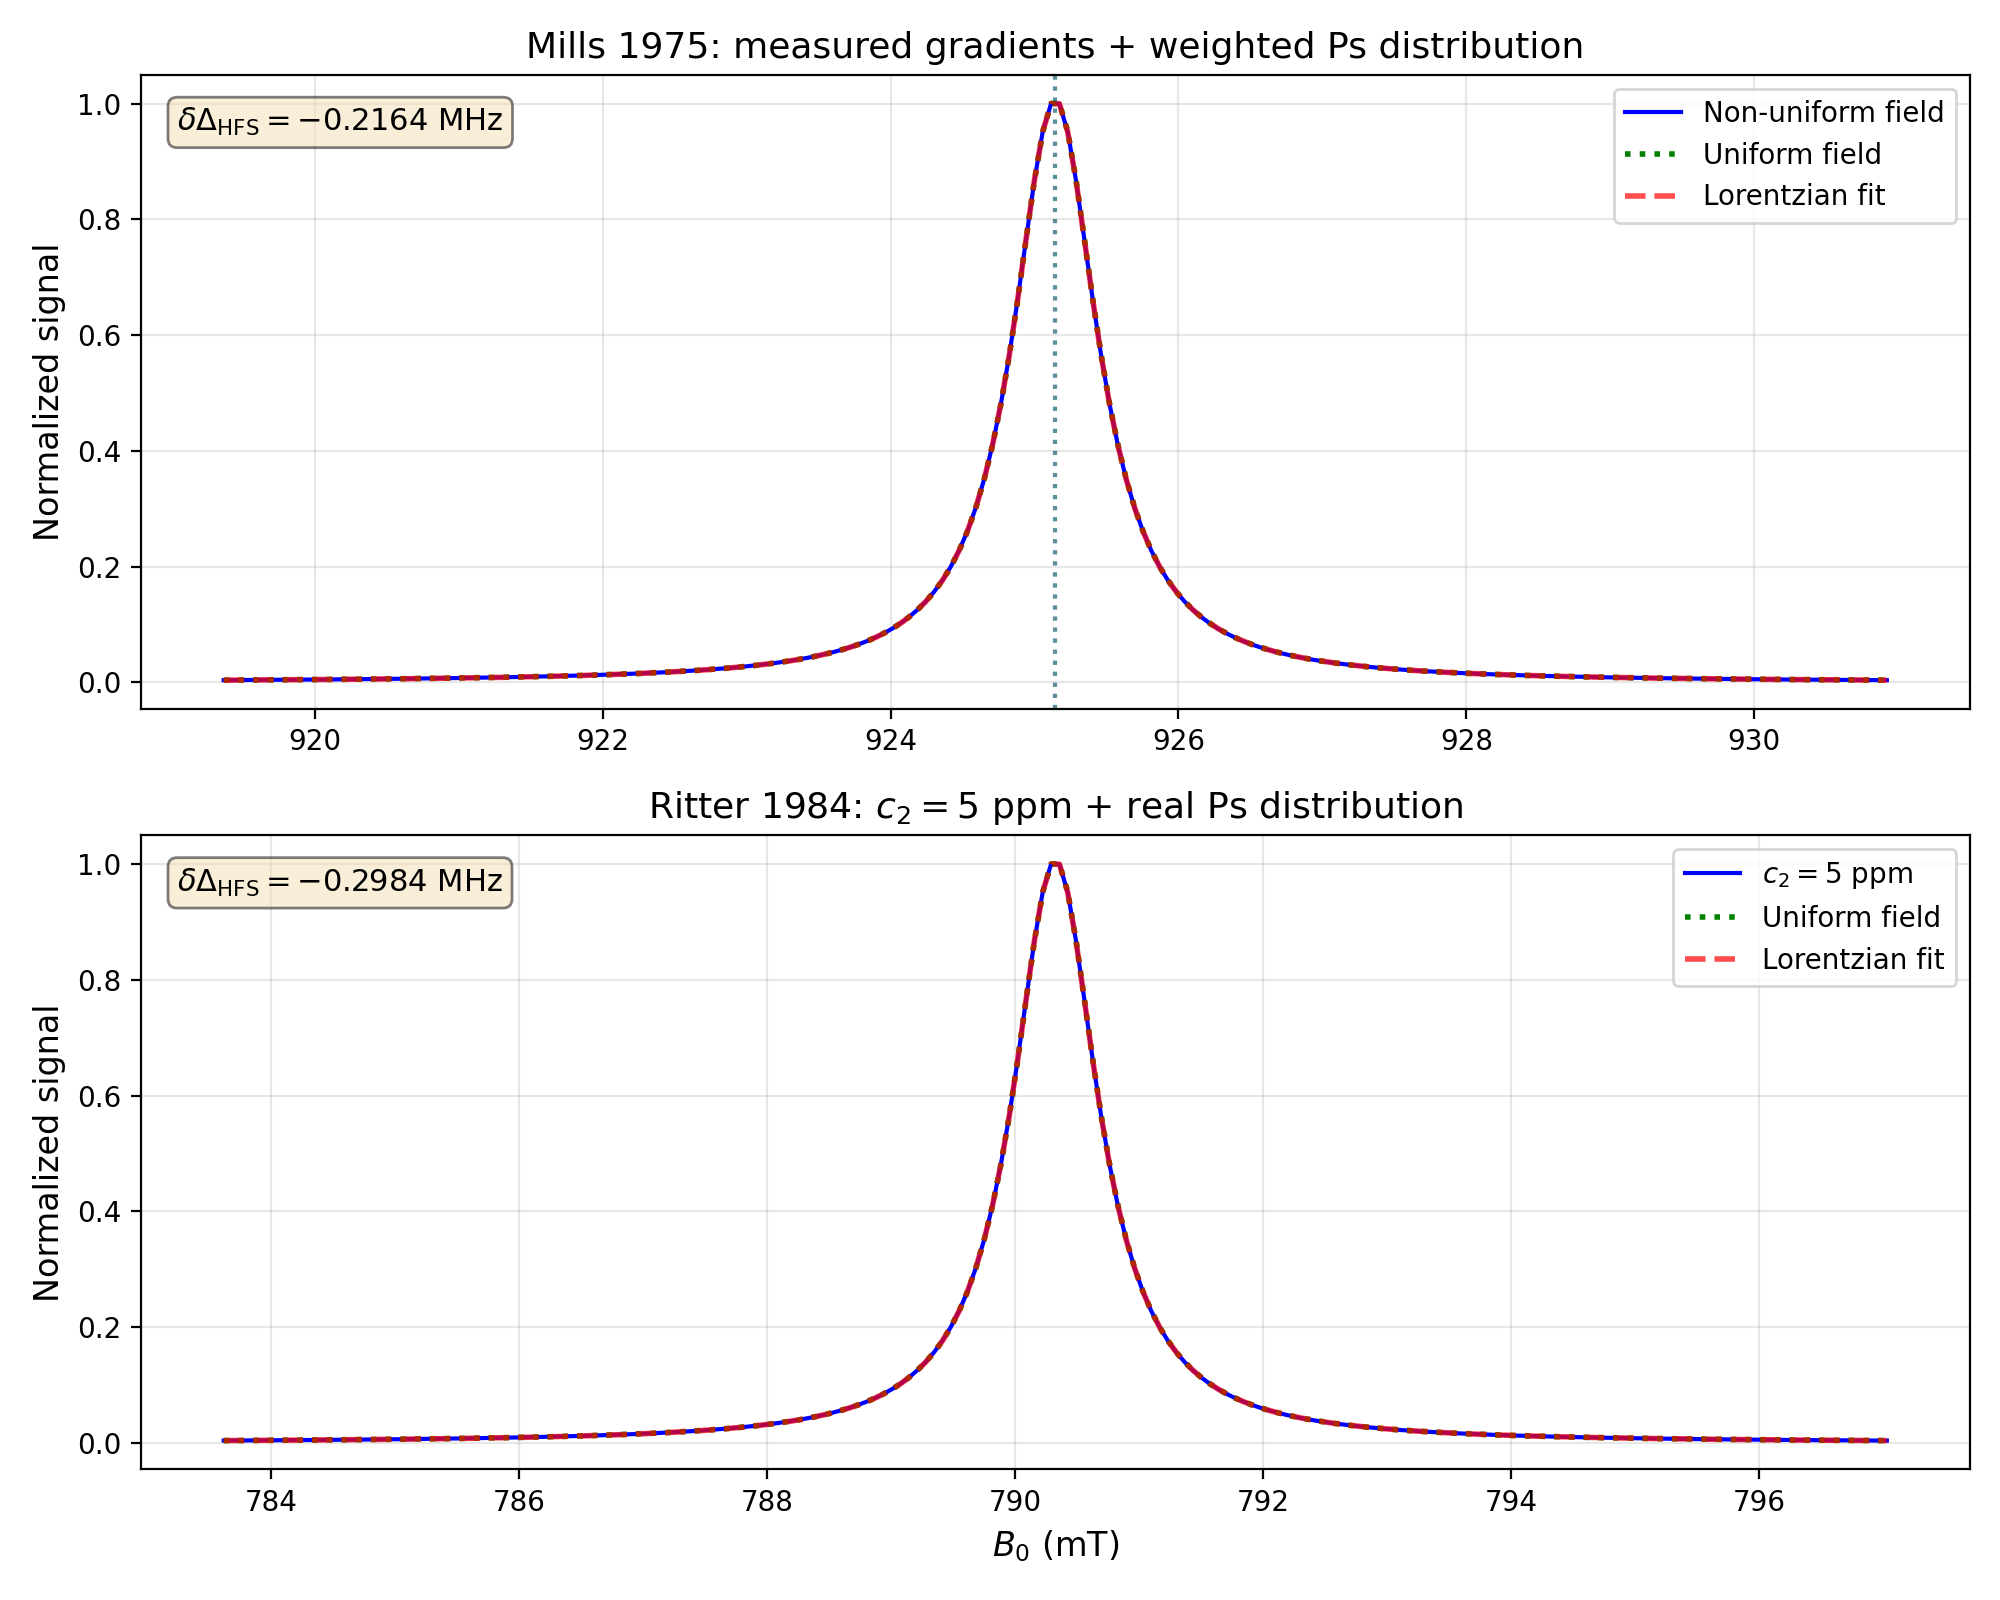
\includegraphics[width=\columnwidth]{resonance_curves_corrected.png}
  \caption{Simulated Zeeman resonance curves with non-uniform magnetic field (blue), Lorentzian fit (red dashed), and uniform-field control (green). Upper panel: Mills configuration with NMR-measured gradients ($\alpha_r = -0.21$\,m$^{-2}$, $\alpha_z = +0.44$\,m$^{-2}$). Lower panel: Ritter configuration with $c_2 = 5$\,ppm. The annotated $\delta\Delta_\mathrm{HFS}$ values are baseline-subtracted.}
  \label{fig:resonance}
\end{figure}

\subsection{Ritter: quadrupolar scan}
\label{sec:ritter_results}

Table~\ref{tab:results} presents $\delta\Delta_\mathrm{HFS}$ for the Ritter configuration as a function of the quadrupolar coefficient $c_2$, using the actual cavity dimensions and positronium confinement region. The shift scales linearly with $c_2$, as expected from the first-order mechanism. For the post-shimming range $c_2 = 3$--$5$\,ppm, the bias is $-0.18$ to $-0.30$\,MHz (Fig.~\ref{fig:ritter_scan}).

\begin{table}[t]
\caption{Systematic shift $\delta\Delta_\mathrm{HFS}$ for each experimental configuration using actual dimensions, field profiles, and positronium distributions from the original publications.}
\label{tab:results}
\begin{ruledtabular}
\begin{tabular}{llr}
Configuration & Parameters & $\delta\Delta_\mathrm{HFS}$ \\
 & & (MHz) \\
\hline
Mills (meas.\ gradients) & Published data & $-0.22$ \\
Ritter ($c_2 = 3$\,ppm) & Post-shimming & $-0.18$ \\
Ritter ($c_2 = 5$\,ppm) & Post-shimming & $-0.30$ \\
Ritter ($c_2 = 10$\,ppm) & Pre-shimming & $-0.60$ \\
Ritter ($c_2 = 20$\,ppm) & Pre-shimming & $-1.19$ \\
Ishida SC (0.9\,ppm) & Uniform Ps & $+0.18$ \\
Ishida SC (0.9\,ppm) & $\lambda = 30$\,mm & $-0.05$ \\
\end{tabular}
\end{ruledtabular}
\end{table}

\begin{figure}[htbp]
  \centering
  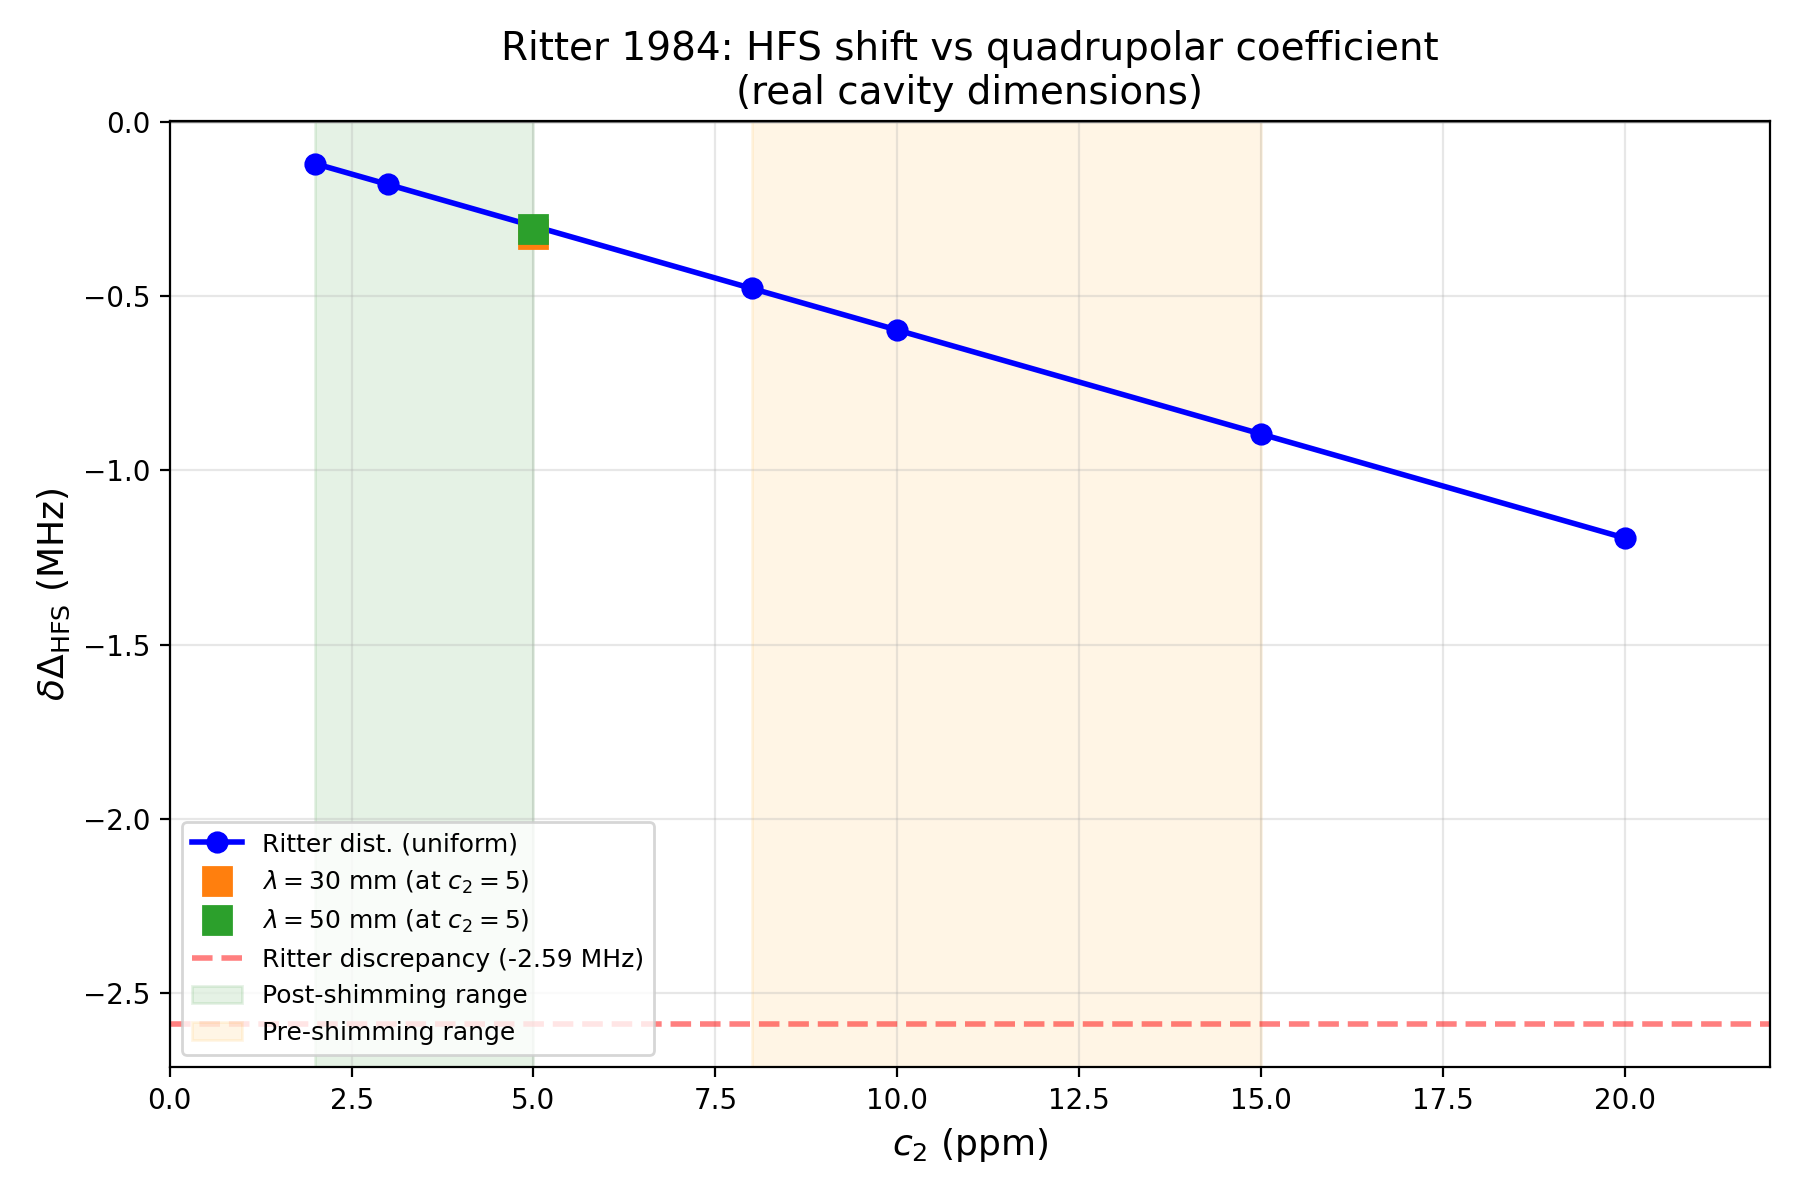
\includegraphics[width=\columnwidth]{ritter_c2_scan.png}
  \caption{Systematic shift for the Ritter configuration with actual cavity dimensions ($R_\mathrm{cav} = 76.8$\,mm, $L_\mathrm{cav} = 38.1$\,mm) and positronium confined to $R = 12.7$\,mm. Green shading: post-shimming range ($c_2 = 2$--$5$\,ppm); orange shading: pre-shimming range. The dashed line marks the Ritter discrepancy ($-2.59$\,MHz).}
  \label{fig:ritter_scan}
\end{figure}

\subsection{Ishida verification}
\label{sec:ishida}

For the Ishida configuration ($B_0 = 0.866$\,T, $\nu_\mathrm{MW} = 2856.6$\,MHz, $R_\mathrm{cav} = 64$\,mm, $L_\mathrm{cav} = 100$\,mm, 0.9\,ppm residual non-uniformity), the simulation gives $\delta\Delta_\mathrm{HFS} = +0.18$\,MHz for uniform Ps and $-0.05$\,MHz for non-thermalized Ps ($\lambda = 30$\,mm). Both values are well below the experimental uncertainty of $\pm 2.1$\,MHz, confirming that the superconducting magnet's high uniformity effectively eliminates this systematic.

\subsection{Comparison with experimental data}
\label{sec:comparison}

Table~\ref{tab:comparison} compares the simulation results with the published measurements. The field-inhomogeneity correction alone accounts for $5\%$ of the Mills discrepancy and $7$--$12\%$ of the Ritter discrepancy. When combined with the $\sim 2$\,MHz non-thermalization correction estimated by Ishida \textit{et~al.}~\cite{Ishida2014}, the total correction reduces the discrepancy from $3.9\sigma$ to approximately $1.5\sigma$.

\begin{table*}[t]
\caption{Comparison with published HFS measurements. $\delta_B$ is the field-inhomogeneity correction from this work. The combined correction adds the Ishida non-thermalization estimate ($\sim 2$\,MHz) to $\delta_B$; these are not strictly additive (see Sec.~\ref{sec:thermalization}).}
\label{tab:comparison}
\begin{ruledtabular}
\begin{tabular}{lcccccc}
 & $\Delta_\mathrm{HFS}$ & Residual & $\delta_B$ & Combined & Final residual & Significance \\
 & (MHz) & (MHz) & (MHz) & (MHz) & (MHz) & \\
\hline
Mills~\cite{Mills1983}  & $203\,387.5 \pm 1.6$ & $-4.19$ & $-0.22$ & $\sim -2.2$ & $\sim -2.0$ & $\sim 1.2\sigma$ \\
Ritter~\cite{Ritter1984} & $203\,389.10 \pm 0.74$ & $-2.59$ & $-0.18$ to $-0.30$ & $\sim -2.2$ & $\sim -0.4$ & $\sim 0.5\sigma$ \\
Ishida~\cite{Ishida2014} & $203\,394.2 \pm 2.1$ & $+2.51$ & $+0.18$ & $\sim +0.2$ & $\sim +2.3$ & $1.1\sigma$ \\
QED~\cite{Kniehl2000,Baker2014} & $203\,391.69 \pm 0.41$ & --- & --- & --- & --- & --- \\
\end{tabular}
\end{ruledtabular}
\end{table*}

%% ====================================================================
\section{Discussion}
\label{sec:discussion}
%% ====================================================================

\subsection{Physical mechanism}

The bias arises from the combination of two effects: (i) the spatial average of the field over the positronium distribution differs from the nominal central value ($\langle B \rangle \neq B_0$), and (ii) the Breit-Rabi inversion is a nonlinear function of $B$. Effect (i) alone produces a first-order shift $\delta\nu \approx (d\nu_\mathrm{trans}/dB)\,\langle\delta B\rangle$. Effect (ii) adds a second-order contribution from the Jensen inequality. In our simulations, the first-order effect dominates.

Crucially, this is a \emph{bias}, not a broadening. As shown in Fig.~\ref{fig:resonance}, the resonance curve retains its Lorentzian shape to high accuracy (fit residuals $< 10^{-3}$), making the effect invisible in the quality of the fit.

\subsection{Relation to the non-thermalization correction}
\label{sec:thermalization}

Our field-inhomogeneity correction ($-0.22$\,MHz for Mills) and the Ishida non-thermalization correction ($\sim 2$\,MHz) are not strictly additive, because the spatial distribution of non-thermalized Ps affects the field sampling. However, the two effects operate through different physical mechanisms: the non-thermalization correction arises from the velocity-dependent gas density shift, while our correction arises from the position-dependent field bias. As a rough estimate, their sum ($\sim 2.2$\,MHz for Mills) would reduce the discrepancy from $-4.19$\,MHz to $\sim -2.0$\,MHz ($\sim 1.2\sigma$). For Ritter, the combined correction of $\sim 2.2$\,MHz would reduce the residual from $-2.59$ to $\sim -0.4$\,MHz ($< 0.5\sigma$). A self-consistent calculation that simultaneously models thermalization dynamics in a non-uniform field is needed to determine the precise combined correction; this is identified as the key direction for future work.

\subsection{Why this effect was not corrected previously}

Mills \& Bearman~\cite{Mills1975} explicitly measured the field gradients and computed the mean field offset over the positronium distribution (their Eq.~4), obtaining $\langle\delta B/B_0\rangle = +0.44$\,ppm. However, they applied this as a correction to $B_0$ only, without propagating it through the nonlinear Breit-Rabi inversion to determine its effect on the extracted $\Delta_\mathrm{HFS}$. Our calculation, using their own weighting function $1 - b|z|$, reproduces $\langle\delta B/B_0\rangle = +0.52$\,ppm (consistent with their $+0.44$\,ppm) and shows that propagating this offset through the nonlinear Breit-Rabi inversion yields a shift of $-0.22$\,MHz---small compared to the statistical uncertainty of their measurement ($\pm 1.6$\,MHz) but a non-negligible contribution to the overall discrepancy when combined with other systematics.

The field-inhomogeneity bias is also independent of gas pressure, so the standard extrapolation to zero gas density does not remove it. Furthermore, the Lorentzian line shape is preserved to high accuracy, so it would not be visible as a line-shape anomaly.

\subsection{Consistency with Ishida}

The superconducting solenoid used by Ishida \textit{et~al.} had 0.9\,ppm field uniformity and a cavity of $R = 64$\,mm. Our simulation confirms $|\delta\Delta_\mathrm{HFS}| < 0.2$\,MHz for this configuration, naturally explaining why their result agrees with QED.

\subsection{Limitations}

The Mills result ($-0.22$\,MHz) uses the published gradients and detection weighting directly. The Ritter result depends on the assumed $c_2$, which is constrained to $3$--$5$\,ppm by their reported 0.5\,ppm post-shimming uniformity. The dominant remaining uncertainty is the interplay between field inhomogeneity and non-thermalization, which requires a self-consistent simulation of positronium thermalization dynamics in a non-uniform magnetic field.

We note that contact patch potentials on the copper cavity walls are negligible for ground-state positronium: the Speake-Trenkel formalism~\cite{Speake2003} shows that the electric fields from micrometer-scale grain boundaries are exponentially suppressed at the cavity center, producing energy shifts of order $10^{-15}$\,eV. We also neglect the non-Hermitian corrections from singlet annihilation, which Mills~\cite{Mills1983} showed produce a line-center shift of $\sim 0.5$\,MHz; this correction largely cancels in our baseline-subtracted result [Eq.~(\ref{eq:shift})].

\subsection{Implications for future measurements}

Our results imply that any future precision measurement of the ground-state positronium HFS must verify the magnetic field uniformity at the $\sim 1$\,ppm level and demonstrate complete Ps thermalization. The ongoing programs at ETH Zurich~\cite{ThorpeWoods2026} and the University of Tokyo should be sensitive to this systematic if conventional magnets are used. The Ramsey spectroscopy techniques being developed at UCL~\cite{Newson2026} introduce new sensitivity to field gradients between the interaction regions, making field characterization even more critical.

%% ====================================================================
\section{Conclusion}
\label{sec:conclusion}
%% ====================================================================

We have quantified for the first time the systematic bias introduced by magnetic field inhomogeneity in the 1983--1984 positronium HFS measurements. Using the field gradients and detection weighting published by Mills \& Bearman, we find $\delta\Delta_\mathrm{HFS} = -0.22$\,MHz for the Mills measurement. For the Ritter measurement, the bias is $-0.18$ to $-0.30$\,MHz, consistent with their more careful field shimming.

These corrections, combined with the $\sim 2$\,MHz non-thermalization systematic identified by Ishida \textit{et~al.}, reduce the $3.9\sigma$ discrepancy to approximately $1.5\sigma$ for the weighted average. For the Ritter measurement alone, the combined correction brings the result into agreement with QED ($< 0.5\sigma$).

The field-inhomogeneity bias uses experimentally measured gradients and naturally vanishes for the Ishida superconducting magnet ($|\delta\Delta_\mathrm{HFS}| < 0.2$\,MHz). A self-consistent treatment combining field inhomogeneity and thermalization dynamics---accounting for the correlated sampling of non-uniform fields by non-thermalized positronium---is the key remaining step toward a definitive resolution.

%% ====================================================================
\begin{acknowledgments}
The simulation code is publicly available at \url{https://github.com/Jefemaestro33/ps-hfs-field-inhomogeneity}.
\end{acknowledgments}
%% ====================================================================

\bibliography{02_paper_refs}

\end{document}
